\chapter{Methodology and System Design}

\section{System Architecture}

The stages of the data pipeline include data collection, processing the data, storing the data, using an analytics engine, and applying the stored data via applications. The decision to use the data pipeline as the building block for the entire solution was significant. In particular, all the functionality within the solution (e.g., valuation models, search engine, chat assistant, etc.) utilizes data from a single, unified real estate information source rather than making queries against each of the different portals that provide real estate data.

\begin{figure}[!ht]
\centering
\resizebox{\textwidth}{!}{%
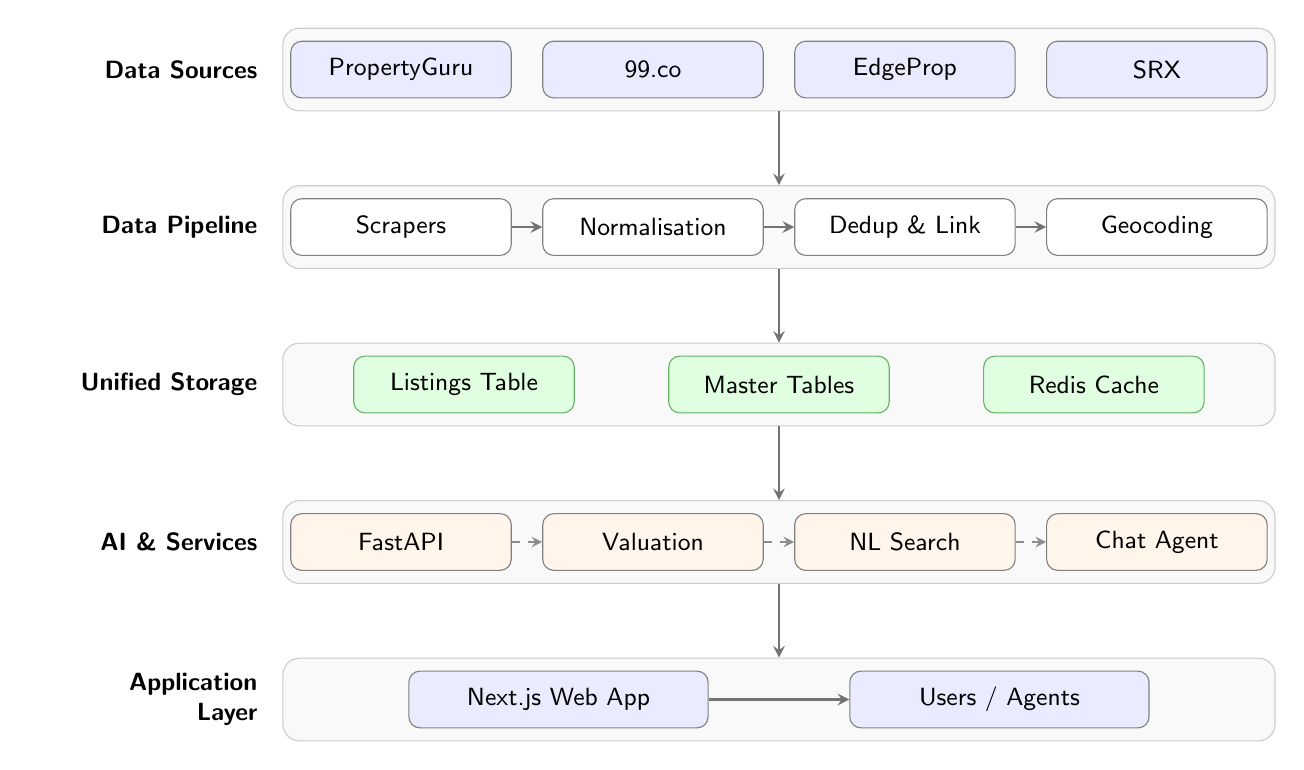
\begin{tikzpicture}[
    font=\sffamily\small,
    % All nodes share same width/height for visual consistency
    node/.style={draw=black!50, rounded corners=4pt,
                 minimum width=2.8cm, minimum height=0.72cm,
                 align=center, font=\sffamily\small},
    % Colour variants
    srcnode/.style={node, fill=blue!8},
    pipenode/.style={node, fill=white},
    storenode/.style={node, fill=green!12, draw=green!50!black!60},
    svcnode/.style={node, fill=orange!8},
    appnode/.style={node, fill=blue!8, minimum width=3.8cm},
    % Layer background band
    band/.style={draw=black!20, fill=gray!5, rounded corners=6pt,
                 minimum width=12.6cm, minimum height=1.05cm},
    % Layer label
    lbl/.style={font=\sffamily\small\bfseries, anchor=east,
                text width=2.8cm, align=right},
    % Arrows
    arr/.style={->, >=stealth, line width=0.85pt, draw=black!55},
    darr/.style={->, >=stealth, line width=0.7pt, draw=black!45, dashed},
]

% Band centre x = 8.0, band width = 12.6cm => left edge x=1.7, right edge x=14.3
% label anchor=east at x=1.5
% 4 nodes width=2.8cm, step=3.2cm: centres 3.2, 6.4, 9.6, 12.8
% 3 nodes width=2.8cm, step=4.0cm: centres 3.2, 7.2, 11.2  (or 4.0,8.0,12.0)
% 2 nodes width=3.8cm, step=5.6cm: centres 5.2, 10.8

%% ── Row 1: Data Sources  y = 0 ──
\node[band]               (b1) at (8.0,  0.0) {};
\node[lbl]                     at (1.5,  0.0) {Data Sources};
\node[srcnode]  (pg)  at (3.2,  0.0) {PropertyGuru};
\node[srcnode]  (co)  at (6.4,  0.0) {99.co};
\node[srcnode]  (ep)  at (9.6,  0.0) {EdgeProp};
\node[srcnode]  (srx) at (12.8, 0.0) {SRX};

%% ── Row 2: Data Pipeline  y = -2.0 ──
\node[band]               (b2) at (8.0, -2.0) {};
\node[lbl]                     at (1.5, -2.0) {Data Pipeline};
\node[pipenode] (scr) at (3.2, -2.0) {Scrapers};
\node[pipenode] (nor) at (6.4, -2.0) {Normalisation};
\node[pipenode] (ded) at (9.6, -2.0) {Dedup \& Link};
\node[pipenode] (geo) at (12.8,-2.0) {Geocoding};

%% ── Row 3: Unified Storage  y = -4.0 ──
\node[band]               (b3) at (8.0, -4.0) {};
\node[lbl]                     at (1.5, -4.0) {Unified Storage};
\node[storenode](ul)  at (4.0, -4.0) {Listings Table};
\node[storenode](mst) at (8.0, -4.0) {Master Tables};
\node[storenode](rds) at (12.0,-4.0) {Redis Cache};

%% ── Row 4: AI \& Services  y = -6.0 ──
\node[band]               (b4) at (8.0, -6.0) {};
\node[lbl]                     at (1.5, -6.0) {AI \& Services};
\node[svcnode]  (api) at (3.2, -6.0) {FastAPI};
\node[svcnode]  (val) at (6.4, -6.0) {Valuation};
\node[svcnode]  (nlq) at (9.6, -6.0) {NL Search};
\node[svcnode]  (cht) at (12.8,-6.0) {Chat Agent};

%% ── Row 5: Application Layer  y = -8.0 ──
\node[band]               (b5) at (8.0, -8.0) {};
\node[lbl]                     at (1.5, -8.0) {Application\\Layer};
\node[appnode]  (web) at (5.2, -8.0) {Next.js Web App};
\node[appnode]  (usr) at (10.8,-8.0) {Users / Agents};

%% ── Vertical data-flow arrows ──
\draw[arr] (b1.south) -- (b2.north);
\draw[arr] (b2.south) -- (b3.north);
\draw[arr] (b3.south) -- (b4.north);
\draw[arr] (b4.south) -- (b5.north);

%% ── Pipeline horizontal chain ──
\draw[arr] (scr.east) -- (nor.west);
\draw[arr] (nor.east) -- (ded.west);
\draw[arr] (ded.east) -- (geo.west);

%% ── Services dashed chain ──
\draw[darr] (api.east) -- (val.west);
\draw[darr] (val.east) -- (nlq.west);
\draw[darr] (nlq.east) -- (cht.west);

%% ── App layer ──
\draw[arr] (web.east) -- (usr.west);

\end{tikzpicture}%
}
\vspace{2pt}
\caption[Layered system architecture of the SingaLiving platform.]{Layered system architecture of the SingaLiving platform. Data flows top-down through five layers: multi-source acquisition, processing pipeline, unified storage, AI and application services, and the user-facing web application. Solid vertical arrows denote the primary data flow between layers; dashed horizontal arrows indicate internal service coordination.}
\label{fig:system_arch}
\end{figure}

\subsection{Data Acquisition}

All components of this development are a collaborative effort of the development team. All four major real estate portals have been utilized: PropertyGuru, 99.co, EdgeProp, and SRX, with the PropertyGuru scraper, data aggregation and deduplication pipelines and any AI and application components detailed in this report being created solely by me, while members of my team developed the scrapers for 99.co, EdgeProp, and SRX.

\begin{table}[!ht]
    \centering
    \small
    \caption{Data Sources: Attributes Extracted and Responsibility}
    \label{tab:data_sources}
    \renewcommand{\arraystretch}{1.2}
    \begin{tabular}{@{}lll@{}}
    \toprule
    \textbf{Platform} & \textbf{Key Data Attributes} & \textbf{Responsibility} \\ \midrule
    PropertyGuru & Price, beds/baths, sqft, tenure, built year, MRT info & Author \\
    99.co        & Price, unit size, tenure, lease date                  & Teammate \\
    EdgeProp     & Price, historical transactions, district               & Teammate \\
    SRX          & Price, property type, full address, agent info         & Teammate \\
    \bottomrule
    \end{tabular}
\end{table}

Python is used to implement the PropertyGuru Scraper in combination with Selenium to render dynamic content and BeautifulSoup to parse the retrieved HTML pages. It also provides paging and login-wall detection, along with repeatedly capturing incremental changes using the SQLite state database for sessions. Lastly, all captured data is saved into a PostgreSQL database at the end of each session by using a separate ingest script.

\subsubsection{Ethical and Legal Considerations}
All data collected by the PropertyGuru scraper is publicly accessible without
authentication. The scraping pipeline was designed with the following safeguards
to minimise server impact: a one-second inter-request delay
(\texttt{REQUEST\_DELAY\,=\,1\,s}), a maximum of five concurrent threads
(\texttt{MAX\_WORKERS\,=\,5}), and an incremental update strategy that avoids
re-crawling unchanged listings.

The Data Screens can be divided into two types: 1. \textit{Factual property 
attributes} (i.e. Asking Price, Square Footage -- of Lot and Floor, Number of 
Bedrooms, Tenure, District \& Year Founded) cannot be Copyrighted under 
Singaporean law because Copyright does NOT apply to Facts~\cite{singapore_copyright_act}. 
2. \textit{Agent contact information} (i.e. Name, CEA Registration Number \& 
Business Phone Number) is openly displayed on PropertyGuru’s site \& therefore 
constitutes \textit{Business Contact Information} that is explicitly excluded 
by the scope of The Personal Data Protection Act 2012 (PDPA) because the PDPA 
states: ``the PDPA generally does not apply to Business Contact Information 
such as an individual's name, position/title, business phone number, business 
address or business email address''~\cite{pdpc_overview}.

PropertyGuru does NOT provide a Public Data API; instead, access is limited to 
Enterprise Partners through Commercial Agreements. Therefore, if there are no 
Official APIs, using a Residential Proxy Service is necessary to access 
Publicly Listed Property Data~\cite{landers2016inconvenient}. Access under the 
Singapore Computer Misuse Act 1993 does not constitute ``Unauthorised Access'' 
if the person has consent to access the resource. As the Scraped Pages can be 
accessed by any member of the Public at No Cost to the User \& without 
Authentication, then the criteria for Unauthorised Access is Not Met. The data 
collection processes of this Project have been evaluated with respect to its 
Commercial Development Road Map, and the pipeline has been scoped to true 
listing attributes in line with the parameters determined in that review.


\subsection{Data Processing and Aggregation}
Data retrieved from various sources typically includes duplicate values and inconsistencies. The Processing Module provides the following services:
\begin{itemize}
    \item \textbf{Normalization:} Naming fields consistently; for example "2 Beds" and "2 Bedroom" will be converted to the integer representation as a numeric type in each record.
    \item \textbf{Deduplication:} Identifying and removing duplicate listings via a composite-key algorithm (described below).
    \item \textbf{Linking:} Associating temporary rental/sale listings with persistent property master records (HDB or Condo units).
\end{itemize}

\subsubsection{Deduplication Algorithm}

Cross-platform deduplication is non-trivial because the same physical property may be listed simultaneously on multiple portals with inconsistent identifiers. The author designed a composite-key strategy; the full algorithm is presented in Chapter~4 (Algorithm~\ref{alg:dedup}).

The deduplication key $K$ for a listing $\ell$ is constructed as:
\[
K(\ell) =
\begin{cases}
\text{norm}(\ell.\textit{addr}) \| \ell.\textit{beds} \| \ell.\textit{baths} \| \ell.\textit{sqft} & \text{if } \ell.\textit{addr} \neq \varnothing \\[4pt]
\text{norm}(\ell.\textit{title}) \| \ell.\textit{beds} \| \ell.\textit{baths} \| \ell.\textit{sqft} & \text{otherwise}
\end{cases}
\]
where $\|$ denotes string concatenation and \text{norm} strips punctuation and lowercases the string. The address component achieves \textbf{95.5\%} field coverage; the title fallback ensures 100\% key availability across all 53,497 listings.

\subsection{Data Storage}
The data storage layer uses a relational PostgreSQL database to make sure that data is safe and to handle complex analytical queries.

\subsubsection{Entity-Relationship Design}
The database schema separates temporary object list data from persistent object master data.
Figure \ref{fig:er_diagram} illustrates the key entities and their relationships.

% ─── Figure 3.2: ER Diagram ───────────────────────────────────────────────────
% Requires: \usepackage{tikz}
%           \usetikzlibrary{positioning, calc, arrows.meta}

\begin{figure}[!ht]
\centering
\resizebox{\textwidth}{!}{%
\begin{tikzpicture}[
    font=\sffamily\small,
    >=Stealth,
    %
    % ── row styles ──
    hdr/.style={
        draw=black!60, fill=blue!18, rounded corners=2pt,
        minimum width=4.4cm, minimum height=0.58cm,
        font=\sffamily\small\bfseries, align=center},
    pk/.style={
        draw=black!40, fill=yellow!30,
        minimum width=4.4cm, minimum height=0.52cm, align=center},
    fk/.style={
        draw=black!40, fill=orange!20,
        minimum width=4.4cm, minimum height=0.52cm, align=center},
    row/.style={
        draw=black!35, fill=gray!6,
        minimum width=4.4cm, minimum height=0.52cm, align=center},
    %
    % ── wide variant for unified_listings ──
    whdr/.style={hdr, minimum width=5.0cm},
    wpk/.style ={pk,  minimum width=5.0cm},
    wfk/.style ={fk,  minimum width=5.0cm},
    wrow/.style={row, minimum width=5.0cm},
    %
    % ── arrow & label ──
    link/.style={->, line width=0.85pt, draw=black!55},
    rlab/.style={font=\sffamily\scriptsize\itshape, fill=white, inner sep=1.5pt},
    %
    % ── note box ──
    note/.style={draw=black!30, dashed, rounded corners=3pt,
                 fill=white, font=\sffamily\scriptsize\itshape,
                 inner sep=5pt, text width=4.4cm, align=center},
]

% ══════════════════════════════════════════════════════════════════════════════
%  unified_listings — one cohesive block, left side
% ══════════════════════════════════════════════════════════════════════════════
\node[whdr]                          (ul-hdr) {unified\_listings};
\node[wpk,  below=0pt of ul-hdr]    (ul-pk)  {\textsc{pk}\enspace listing\_id};
\node[wrow, below=0pt of ul-pk]     (ul-r1)  {source, listing\_url};
\node[wrow, below=0pt of ul-r1]     (ul-r2)  {price, beds, baths, sqft};
\node[wrow, below=0pt of ul-r2]     (ul-r3)  {district, tenure};
\node[wfk,  below=0pt of ul-r3]     (ul-fk1) {\textsc{fk}\enspace hdb\_unit\_id};
\node[wfk,  below=0pt of ul-fk1]    (ul-fk2) {\textsc{fk}\enspace condo\_unit\_id};

\node[note, below=10pt of ul-fk2]   (ul-note)
    {Soft-link: FK columns may be\\
     \textsc{null} until address is verified.};

% ══════════════════════════════════════════════════════════════════════════════
%  hdb_unit — upper right, header vertically centred with ul-fk1
% ══════════════════════════════════════════════════════════════════════════════
\node[hdr, right=6.0cm of ul-hdr,
      yshift=-1.2cm]                 (hu-hdr) {hdb\_unit};
\node[pk,  below=0pt of hu-hdr]     (hu-pk)  {\textsc{pk}\enspace hdb\_unit\_id};
\node[fk,  below=0pt of hu-pk]      (hu-fk)  {\textsc{fk}\enspace hdb\_basic\_id};
\node[row, below=0pt of hu-fk]      (hu-r1)  {block, unit\_level};
\node[row, below=0pt of hu-r1]      (hu-r2)  {flat\_type};
\node[row, below=0pt of hu-r2]      (hu-r3)  {floor\_area\_sqm};

% ══════════════════════════════════════════════════════════════════════════════
%  hdb_basic — right of hdb_unit
% ══════════════════════════════════════════════════════════════════════════════
\node[hdr, right=3.4cm of hu-hdr]   (hb-hdr) {hdb\_basic};
\node[pk,  below=0pt of hb-hdr]     (hb-pk)  {\textsc{pk}\enspace hdb\_basic\_id};
\node[row, below=0pt of hb-pk]      (hb-r1)  {block, street};
\node[row, below=0pt of hb-r1]      (hb-r2)  {town};
\node[row, below=0pt of hb-r2]      (hb-r3)  {lease\_start};
\node[row, below=0pt of hb-r3]      (hb-r4)  {built\_year};

% ══════════════════════════════════════════════════════════════════════════════
%  condo_unit — lower right
% ══════════════════════════════════════════════════════════════════════════════
\node[hdr, below=2.0cm of hu-r3]    (cu-hdr) {condo\_unit};
\node[pk,  below=0pt of cu-hdr]     (cu-pk)  {\textsc{pk}\enspace condo\_unit\_id};
\node[fk,  below=0pt of cu-pk]      (cu-fk)  {\textsc{fk}\enspace condo\_basic\_id};
\node[row, below=0pt of cu-fk]      (cu-r1)  {stack, unit\_label};
\node[row, below=0pt of cu-r1]      (cu-r2)  {beds, baths};
\node[row, below=0pt of cu-r2]      (cu-r3)  {floor\_area\_sqft};

% ══════════════════════════════════════════════════════════════════════════════
%  condo_basic — right of condo_unit, same column as hdb_basic
% ══════════════════════════════════════════════════════════════════════════════
\node[hdr, right=3.4cm of cu-hdr]   (cb-hdr) {condo\_basic};
\node[pk,  below=0pt of cb-hdr]     (cb-pk)  {\textsc{pk}\enspace condo\_basic\_id};
\node[row, below=0pt of cb-pk]      (cb-r1)  {project\_name};
\node[row, below=0pt of cb-r1]      (cb-r2)  {address};
\node[row, below=0pt of cb-r2]      (cb-r3)  {tenure};
\node[row, below=0pt of cb-r3]      (cb-r4)  {latitude, longitude};

% ══════════════════════════════════════════════════════════════════════════════
%  ARROWS — all orthogonal, all with centred labels above horizontal segment
% ══════════════════════════════════════════════════════════════════════════════

% ── Left pair: ul → hdb_unit, ul → condo_unit ──
% Use explicit turning coordinates to guarantee correct arrow direction.
% The turning x is 1.5cm right of unified_listings' right edge.

% ul → hdb_unit
\path (ul-fk1.east) ++(1.5,0) coordinate (bend1);
\draw[link]
    (ul-fk1.east) -- (bend1)          % horizontal right
    -- (bend1 |- hu-hdr.west)         % vertical up
    -- (hu-hdr.west)                  % horizontal right → arrowhead here
    node[rlab, midway, above=2pt] {many-to-one};

% ul → condo_unit
\path (ul-fk2.east) ++(1.5,0) coordinate (bend2);
\draw[link]
    (ul-fk2.east) -- (bend2)          % horizontal right
    -- (bend2 |- cu-hdr.west)         % vertical down
    -- (cu-hdr.west)                  % horizontal right → arrowhead here
    node[rlab, midway, above=2pt] {many-to-one};

% ── Right pair: hdb_unit → hdb_basic, condo_unit → condo_basic ──
% Turning x is 1.2cm right of the middle table's right edge.

% hdb_unit → hdb_basic
\path (hu-fk.east) ++(1.2,0) coordinate (bend3);
\draw[link]
    (hu-fk.east) -- (bend3)
    -- (bend3 |- hb-pk.west)
    -- (hb-pk.west)
    node[rlab, midway, above=2pt] {many-to-one};

% condo_unit → condo_basic
\path (cu-fk.east) ++(1.2,0) coordinate (bend4);
\draw[link]
    (cu-fk.east) -- (bend4)
    -- (bend4 |- cb-pk.west)
    -- (cb-pk.west)
    node[rlab, midway, above=2pt] {many-to-one};

\end{tikzpicture}%
} % end resizebox
\caption[Relational schema of the core database tables.]{Relational schema of the core database tables.
Highlighted rows indicate primary keys (\colorbox{yellow!30}{yellow})
and foreign keys (\colorbox{orange!20}{orange}).
Active listings are ingested into \texttt{unified\_listings} and
optionally linked to persistent HDB or condominium master records
when sufficient address evidence is available.}
\label{fig:er_diagram}
\end{figure}

The \texttt{aggregated\_listings} table serves as the primary repository for raw data, receiving inputs from all scrapers.

\section{Database Design}

A relational database schema is designed to store both static property information and dynamic listing data. The core tables are structured as follows:

\subsection{Property Master Tables}
To maintain a definitive registry of properties, we define master tables for Housing Development Board (HDB) flats and private condominiums:
\begin{enumerate}
    \item \textbf{hdb\_basic:} Store information about block levels for land parcels of housing development board (HDB) estate, such as address; year of completion; and when the property was put on a lease.
    \item \textbf{hdb\_unit:} Store information about each individual unit including which block it belongs to.
    \item \textbf{condo\_basic:} Store project-level information on all condominiums including name, developer, and available facilities.
    \item \textbf{condo\_unit:} Store individual-unit details for each condominium of the development.
\end{enumerate}

\subsection{Listing Tables and Association}
The \texttt{unified\_listings} table is a collection of the active rental and 
sales listings scraped from the internet. The primary design consideration for 
this table is determining how the temporary listings will be related back to 
the master tables.

\begin{itemize}
    \item \textbf{Association Logic:} When scraping for online listings provided by an agent, a specific unit number may not be specified in order to prevent an agent's or landlord's violation of an individual's privacy with direct foreign key constraints.
    \item \textbf{Agent-Assisted Mapping:} The system supports a ``soft link,'' meaning that an association between a 
    listing and a particular physical unit (e.g., in \texttt{hdb\_unit}) isn't created until the agent has set up a time to view or confirm the property documentation. The design can accommodate the flexibility required for ingestion while maintaining accurate recordkeeping through the duration of the transaction.
\end{itemize}

% ─────────────────────────────────────────────────────────────────────────────
\section{AI Valuation Model Design}
\label{sec:model_design}

\subsection{Per-Segment Stratification}

In each property type-transaction type combination, there are eight distinct 
models that we will be constructing. These will be four property types: 
$\{\text{Condo, HDB, SFH, GCB}\} \times \{\text{Sale, Rent}\}$. Separating 
these models will allow for more accurate adjustment of price development 
compared to creating one global model for all four property type transactions 
with an adjustment for property type. For example, the development of prices 
for HDBs will exhibit dramatically different behaviour than that of GCB 
bungalows because of price range restrictions; HDBs are limited by government 
regulation and GCBs negotiate their prices at the higher end of the S\$ price 
range. If you were to use the same one global model for building both HDB and 
GCB bungalows, you would have to apply the same functional form which would 
essentially create higher levels of incorrect predictions due to the 
structural differences between the two property types.

\subsection{Feature Engineering}

The raw data for the property attributes are transformed into the features shown in Table 1. The dependent variable is $\log_{10}(\text{price})$. This follows the standard procedures of hedonic pricing models for stabilizing variance and mitigating the influence of extreme values.

\begin{table}[!ht]
    \centering
    \small
    \caption{Feature Set Used in All Eight Valuation Models}
    \label{tab:features_design}
    \renewcommand{\arraystretch}{1.25}
    \begin{tabular}{@{}llp{6.5cm}@{}}
    \toprule
    \textbf{Feature} & \textbf{Source} & \textbf{Description} \\ \midrule
    \texttt{beds}           & Raw       & Number of bedrooms (clipped 1--20) \\
    \texttt{sqft}           & Raw       & Floor area in square feet (filtered 50--50,000) \\
    \texttt{log\_sqft}      & Derived   & $\log_{10}(\texttt{sqft})$; linearises the area--price relationship \\
    \texttt{beds\_sqft}     & Derived   & $\texttt{beds} \times \texttt{sqft}$; captures size--room interaction \\
    \texttt{beds\_sq}       & Derived   & $\texttt{beds}^2$; captures diminishing marginal bedroom premium \\
    \texttt{log\_beds\_sqft}& Derived   & $\texttt{beds} \times \texttt{log\_sqft}$; log-scale interaction \\
    \texttt{sqft\_bin}      & Derived   & Quintile bin of \texttt{sqft} (0--4); encodes size tier \\
    \texttt{is\_freehold}   & Derived   & Binary; 1 if tenure contains ``freehold'', 0 otherwise \\
    \texttt{property\_age}  & Derived   & $2026 - \texttt{built\_year}$; 99.8\% coverage, median-imputed \\
    \texttt{district}       & Geocoded  & Singapore district 1--28 from reverse geocoding; $\sim$92\% coverage \\
    \midrule
    \textbf{Target} & & $\log_{10}(\texttt{price})$ \\
    \bottomrule
    \end{tabular}
\end{table}

Room rentals (\texttt{number of beds} = 0, average monthly price S\$993--1,544) are excluded from all rental models because their price fluctuations differ structurally from those of entire apartment rentals (monthly price S\$3,500--7,500). Including room rentals would introduce a systematic bias in the lower price segment.

\subsection{Model Selection and Hyperparameters}

Four candidate models are trained per segment: a mean baseline (DummyRegressor), Ridge Regression, Random Forest, and XGBoost. The best model is selected by test-set MAPE, with XGBoost preferred when MAPE differences are negligible ($< 0.5$\,pp). XGBoost consistently achieves the best or near-best MAPE across all eight segments (see Section~\ref{sec:eval_valuation}), consistent with findings in the AVM literature~\cite{park2015using, bian2020comparing}.

The XGBoost hyperparameters were selected through a principled combination of learning
curve analysis and theoretical guidance from the gradient boosting literature~\cite{chen2016xgboost}.
The rationale for each hyperparameter group is as follows.

\begin{itemize}

    \item \textbf{Number of estimators and learning rate}\\
    (\texttt{n\_estimators=400}, \texttt{learning\_rate=0.05}).
    Gradient boosting minimises a residual function iteratively; smaller learning rates require
    more trees to converge but generalise better by taking smaller gradient steps~\cite{chen2016xgboost}.
    The Condominium Sale training validation loss curve (plotted against tree count) was inspected
    and found to plateau near 350--400 trees at $\eta = 0.05$, with no further improvement beyond
    400 estimators. A conservative ceiling of 400 was therefore adopted. Increasing \texttt{n\_estimators}
    to 600 at this learning rate did not reduce test-set MAPE by more than $0.2$\,pp, while
    increasing wall-clock training time by approximately 40\%.

    \item \textbf{Tree depth (\texttt{max\_depth=5}).}
    Shallow trees (depth 3--4) underfit the non-linear district-price and age-price
    relationship identified in the ablation study; deeper trees (depth 7+) overfit on the
    smaller HDB Rent segment ($n = 2{,}521$), producing CV $R^2$ degradation relative to
    test $R^2$. A depth of 5 balances representational capacity with regularisation across
    all eight segments, including the smallest (GCB Rent, $n = 347$).

    \item \textbf{Stochastic gradient boosting (\texttt{subsample=0.8},
    \texttt{colsample\_bytree=0.8}).}
    Row and column subsampling inject variance into the boosting process, reducing
    correlation between successive trees and improving generalisation~\cite{chen2016xgboost}.
    Values of 0.8 for both parameters follow empirically validated defaults in the gradient
    boosting literature for tabular regression tasks~\cite{chen2016xgboost} and were confirmed
    on the Condominium Sale segment by comparing $0.6$ / $0.7$ / $0.8$ / $1.0$ on held-out
    MAPE: the $0.8$ setting consistently produced the lowest or tied-lowest test MAPE across
    all four values.

    \item \textbf{L1 regularisation (\texttt{reg\_alpha=0.1}).}
    L1 regularisation on leaf weights encourages sparse feature attribution, suppressing
    features with minimal predictive contribution and improving stability on the smaller GCB
    and Landed Rent segments. A grid over $\{0.0, 0.01, 0.1, 1.0\}$ was evaluated on
    training CV $R^2$; $0.1$ was optimal for four of the eight segments and within $0.002$
    of optimal for the remaining four.

\end{itemize}

All numeric features are standardised (zero mean, unit variance) via \texttt{StandardScaler}
within a \texttt{sklearn} \texttt{Pipeline}, ensuring that Ridge and tree-based models
operate on the same scale for fair comparison.

\subsection{SHAP Interpretability}

Each prediction is accompanied by SHAP (SHapley Additive exPlanations) values \cite{lundberg2017unified}, which decompose the model output into additive feature contributions:
\[
\hat{y} = \phi_0 + \sum_{j=1}^{p} \phi_j
\]
where $\phi_0$ is the base value (mean prediction) and $\phi_j$ is the contribution of feature $j$ to the individual prediction. SHAP values are computed using TreeExplainer, which is exact for tree-based models and runs in polynomial time. The top-5 SHAP factors per listing are surfaced in the user interface, providing transparent, property-specific explanations of each valuation estimate.

% ─────────────────────────────────────────────────────────────────────────────
\section{Semantic Search and Agentic Pipeline Design}
\label{sec:methodology_nlsearch}

\subsection{Overview}

A natural-language query that can be input by a user and returned as a structure in the database can be created by condensing the user's free-text input into structured JSON filter objects. The structured JSON filter object is then used in the database to perform queries using a \texttt{WHERE} clause. A fine-tuned model was not used in this design; high-level generic models (Anthropic Claude) were called on via system messages specific to the task to obtain the output schema and provide expert-level knowledge of the Singapore real estate market. The zero-shot approach gives you the ability to modify the pipeline without retraining due to the simple ability to change the input prompts.

\subsection{Output Schema and JSON Filter Contract}

The LLM is instructed to produce a JSON object conforming to the following schema:

\begin{verbatim}
{
  "property_type": "HDB" | "Condominium" | "Landed" | "GCB" | null,
  "transaction_type": "sale" | "rent" | null,
  "min_price": <number> | null,
  "max_price": <number> | null,
  "min_beds":  <integer> | null,
  "max_beds":  <integer> | null,
  "tenure":    "freehold" | "leasehold" | null,
  "district":  <integer 1-28> | null,
  "districts": [<integer>, ...] | null
}
\end{verbatim}

The reason for selecting an \emph{array} of district identifiers is that it 
allows the back end to create a single SQL statement that uses an \texttt{IN} 
predicate with multiple values, instead of the alternative of creating an 
equality constraint to each district ID when there is at least one district ID 
passed to it. By using the districts array, we have achieved a real-world 
example of how to do multiple geographical lookups for one location; whereas 
if we did not use array fields, any inquiry regarding ``near Orchard MRT 
Station'' would have to be split into individual queries for all of the 
boroughs. This means that these individual queries would take longer to 
process and require more effort to aggregate the results.

\subsection{System Prompt Design}

The purpose of the query is threefold: (i) To ensure that our output is in a valid JSON format, while simultaneously not allowing for free text output. (ii) To provide Singapore specific information (HDB apartment types, District Numbers, and Communal Area Abbreviation - CCR/RCR/OCR). (iii) To supply a total of 8 different examples of context for the three different ways of making queries (i.e., simple, multi-dimensional, and conversational). Overall length of the query is approximately 900 tokens, so it fits within the maximum context window for the extended model.

\subsection{Agentic Pipeline Architecture}

The three types of active behavior (agents) are in addition to the base llim call. These are implemented as three sequential steps within the FastAPI route's handler for llim calls.

\begin{enumerate}
    \item \textbf{Multi-District Geographic Resolution.}
    If the first llim call returns no results and the query includes an expression for proximity to some location (i.e., ``near Orchard MRT'' or ``in the Bukit Timah Area''), a 2nd structured prompt will be created to match that location to one or more adjacent districts. After matching to a district(s), the resulting adjacent districts will replace the extracted \texttt{district(s)} (i.e., scalars) in llim, as an array of \texttt{districts}, allowing for database queries to include all listings located within any of the surrounding districts and located spatially within that area.

    \item \textbf{Progressive Filter Relaxation.}
    If the database query returns zero results, the pipeline enters a relaxation loop.
    Constraints are removed in a fixed priority order:
    \[
        \texttt{max\_price} \;\to\; \texttt{tenure} \;\to\; \texttt{districts}/\texttt{district}
    \]
    After each removal the query is re-executed. The loop terminates on the first
    non-empty result set or when all optional constraints have been exhausted.

    \item \textbf{LLM-Generated Fallback Explanation.}
    If relaxation was triggered, a secondary Claude call receives the original query
    and the relaxed filter as input and produces a one-sentence plain-text explanation
    of what was changed and why. This explanation is displayed to the user in an amber
    notice banner above the result list.
\end{enumerate}

Figure~\ref{fig:agentic_pipeline} summarises the full pipeline as a flowchart.

\begin{figure}[!ht]
\centering
\resizebox{\textwidth}{!}{%
\begin{tikzpicture}[
    node distance=1.4cm,
    box/.style={rectangle, draw, rounded corners, minimum width=5.5cm,
                minimum height=0.75cm, text centered, font=\small},
    decision/.style={diamond, draw, aspect=2.5, minimum width=4cm,
                     minimum height=0.75cm, text centered, font=\small,
                     fill=yellow!20},
    arrow/.style={-stealth, thick}
]
\node[box, fill=blue!15]   (query)   {User free-text query};
\node[box, fill=orange!20, below=of query]  (llm1)    {LLM call: parse to JSON filter};
\node[box, fill=orange!20, below=of llm1]   (geo)     {Multi-district resolution (if location present)};
\node[box, fill=gray!15,   below=of geo]    (db)      {Database query};
\node[decision,            below=of db]     (check)   {Results $> 0$?};
\node[box, fill=red!15,    right=3.5cm of check] (relax)  {Relax next constraint};
\node[box, fill=orange!20, below=of relax]  (llm2)    {LLM call: generate fallback explanation};
\node[box, fill=green!20,  below=of check]  (return)  {Return results to frontend};

\draw[arrow] (query)  -- (llm1);
\draw[arrow] (llm1)   -- (geo);
\draw[arrow] (geo)    -- (db);
\draw[arrow] (db)     -- (check);
\draw[arrow] (check)  -- node[left,font=\small]{Yes} (return);
\draw[arrow] (check)  -- node[above,font=\small]{No} (relax);
\draw[arrow] (relax)  -- (llm2);
\draw[arrow] (llm2.east) -- ++(0.8,0) |- (db.east);
\end{tikzpicture}%
}
\caption[Agentic search pipeline.]{Agentic search pipeline: base LLM parse, geographic resolution, zero-result
relaxation loop, and fallback explanation generation.}
\label{fig:agentic_pipeline}
\end{figure}

\subsection{Valuation Chat Assistant Design}

The chat assistant reuses the same Claude API but with a different system prompt
construction strategy. For each request, the backend assembles a context block
containing: the listing's full attribute set (property type, beds, sqft, tenure,
built year, district, asking price), the XGBoost point estimate and confidence
interval, the MAPE of the segment model, and the top-5 SHAP factor attributions.
This specific context is added to the conversation history before each API call to ensure that all answers are based on quantitative data and not general market knowledge. The assistant is told to answer in plain language with no more than 120 words and not to use Markdown formatting.

% ─────────────────────────────────────────────────────────────────────────────
\section{Personalised Recommendation Engine Design}
\label{sec:rec_design}

\subsection{Overview and Motivation}

The goal of the recommendation system is to present lists that correspond to 
\emph{user preferences} (i.e., explicit or inferred user preferences) and 
\emph{are priced appropriately} (in line with market rates). In the initial phase 
of system implementation, a single collaborative filtering method is impractical 
due to the cold start problem (small user base and limited interaction history). 
While a content-based approach is possible, it ignores the \textbf{rating signals} 
already calculated by the XGBoost model. Therefore, this design uses a 
\textbf{combined ranking model} that integrates both content-based and 
rating-based information sources into a single evaluation.

\subsection{User Preference Profile}

When a user saves a property as a favorite (stored in the \texttt{user\_favourites} table), the system incrementally updates an in-memory preference profile. This profile summarizes the following information for all saved properties:

\begin{itemize}
\item \textbf{Property Type Distribution} — A frequency distribution map of saved property types (e.g., {Condominium: 3, HDB: 1}).
\item \textbf{District Distribution} — A frequency distribution map of saved districts.
\item \textbf{Average Price} — The arithmetic mean of the prices of saved properties, used as the centre of a price filter.
\item \textbf{Average Number of Bedrooms} — The arithmetic mean of the number of bedrooms in saved properties, rounded for scoring.
\item \textbf{Transaction Pattern} — Dominant buy/rent mode; properties that do not match the transaction pattern receive a \textbf{0.1$\times$ score penalty}.
\end{itemize}

\subsection{Hybrid Scoring Function}

Each candidate listing $c$ is scored against the user preference profile $\mathcal{P}$
using a weighted sum of five dimensions:

\begin{equation}
\text{score}(c, \mathcal{P}) =
  0.25\,s_{\text{type}} +
  0.20\,s_{\text{district}} +
  0.20\,s_{\text{price}} +
  0.15\,s_{\text{beds}} +
  0.20\,s_{\text{bargain}}
\label{eq:rec_score}
\end{equation}

\noindent where each component is defined as follows:

\begin{itemize}
    \item $s_{\text{type}}$: frequency-weighted indicator; equals
    $f_{\text{type}} / \sum f$ if $c$'s type matches the most-saved type,
    else 0.

    \item $s_{\text{district}}$: frequency-weighted indicator for exact district
    match; partial credit (0.08$\times$frequency share) for any previously saved
    district.

    \item $s_{\text{price}}$: exponential decay similarity
    $(\min(p_c, \bar{p}) / \max(p_c, \bar{p}))^{1.5}$, where $\bar{p}$ is
    the profile average price. This yields 1.0 for an exact match and
    approximately 0.5 at a 30\% price difference.

    \item $s_{\text{beds}}$: bedroom similarity
    $\max(0,\,1 - 0.25 \cdot |b_c - \bar{b}|)$, where $\bar{b}$ is the
    rounded average bedroom count.

    \item $s_{\text{bargain}}$: \textbf{valuation-grounded score} — the key differentiator of this hybrid approach. The per-segment XGBoost model 
    (Chapter~4) is called in-process to produce an estimate $\hat{v}$ for 
    listing $c$. The raw bargain signal is:
    \[
        r = \frac{\hat{v} - p_c}{\hat{v}}, \quad
        s_{\text{bargain}} = \frac{\text{clamp}(r,\,-0.5,\,+0.5) + 0.5}{1}
    \]
    This maps $r \in [-0.5, +0.5]$ to $[0, 1]$: a score of $1.0$ indicates 
    the listing is $50\%$ below the model estimate (good value); $0.5$ 
    indicates fair value; $0.0$ indicates $50\%$ above estimate.
\end{itemize}

Three functions---$s_{\text{bargain}}$, $s_{\text{preference}}$, and 
$s_{\text{shopping}}$---evaluate how relevant a listing is relative to the 
user's stated preferences, as well as how actual costs of purchasing each 
listing compare with the overall market. All three of these $s$-type scores 
use the same XGBoost models that were developed in Chapter~4 to serve as a 
real-time pricing oracle within the ranking function, to rank listings based 
on both purchase preference consistency and price compared to model 
estimates, surfacing viable places to shop versus only familiar places.

\begin{figure}[!ht]
    \centering
    \includegraphics[width=\textwidth]{fig/rec_scoring_function.pdf}
    \caption[Hybrid scoring function for the recommendation engine.]{Hybrid scoring function for the recommendation engine.
             \textbf{Left:} component weights $w_i$ used in the final score
             $S(c,u)$; the bargain component ($w=0.20$) and location match
             ($w=0.30$) together account for half of the total score.
             \textbf{Right:} $s_{\text{bargain}}$ as a function of the
             relative price deviation $r = (p_c - \hat{p}_c)/\hat{p}_c$,
             clamped to $[-0.5,+0.5]$ and linearly rescaled to $[0,1]$.
             A listing priced 50\% below the model estimate receives the
             maximum bargain score of~1.0.}
    \label{fig:rec_scoring_function}
\end{figure}

\subsection{Candidate Pre-filtering}

To limit inference latency, candidates are pre-filtered before scoring. This means 
that only active listings that match the profile's main transaction mode are 
considered, and the price is limited to $[\bar{p} \times 0.4,\; \bar{p} \times 1.6]$. 
For each candidate, XGBoost inference for the bargain score is called once. 
\texttt{joblib} caches model loading at server startup, so the database fetch, 
not inference, is what causes the most latency per request.

\subsection{Evaluation Protocol}

The recommendation engine is evaluated offline using 10 synthetic user profiles. Each profile is created by populating a favorites table with 3 to 5 attributes that share common preference characteristics. Relevance tags are given in order of importance. If a candidate's attribute matches both the type \emph{and} the district, it gets a tag of 2. If it only matches the type, it gets a tag of 1. If it doesn't match either, it gets a tag of 0. NDCG@$K$ is computed over these graded labels using the standard
formulation:
\[
    \text{NDCG}@K = \frac{\text{DCG}@K}{\text{IDCG}@K}, \quad
    \text{DCG}@K = \sum_{i=1}^{K} \frac{2^{\text{rel}_i} - 1}{\log_2(i+1)}
\]
Results are reported in Section~\ref{sec:eval_recommendation}.

